% This file is the user manual for the UGKS1D and UGKS2D code
%
% Copyright (C) 2012 Wang Ruijie <lainme993@gmail.com> 
%
% Permission is granted to copy, distribute and/or modify this document
% under the terms of the GNU Free Documentation License, Version 1.3 or
% any later version published by the Free Software Foundation; with no
% Invariant Sections, with no Front-Cover Texts, and with no Back-Cover
% Texts.  A copy of the license is included in the section entitled
% ``GNU Free Documentation License.''

\documentclass[a4paper]{book}
\usepackage{hyperref}
\usepackage{parskip}
\usepackage{amsmath,amssymb}
\usepackage{fullpage}
\usepackage{appendix}
\usepackage{graphicx,subfigure}
\usepackage{xcolor}

%no indention
\setlength\parindent{0pt}

%define colors
\definecolor{orange}{HTML}{FF7F00}

%tikz package
\usepackage{tikz}
\usetikzlibrary{positioning,calc}
\usetikzlibrary{arrows,shapes}
\tikzstyle{block} = [rectangle,rounded corners,thin,align=center,fill=green!20,draw=black!20]
\tikzstyle{line} = [-latex]

%define command
\newcommand{\appxchapter}[2][\@empty]{
    \ifx\@empty#1
    \chapter{Appendix \Alph{chapter}: #2}
    \else
    \chapter[#1]{Appendix \Alph{chapter}: #2}
    \fi
}

\newcommand{\hi}[1]{
    \textbf{\textcolor{orange}{#1}}
}

%optionally load package for code highlighting
\IfFileExists{minted.sty} {
    \usepackage{minted}
}{
    \usepackage{listings}
    \lstset{language=[90]Fortran,
        basicstyle=\ttfamily,
        keywordstyle=\color{red},
        commentstyle=\color{green},
        morecomment=[l]{!}
    }
    \lstset{language=sh,
        basicstyle=\ttfamily,
        keywordstyle=\color{red},
        commentstyle=\color{green},
        morecomment=[l]{\#}
    }
    \lstnewenvironment{minted}[2][] {\lstset{language=#2}}{}
}

\begin{document}
%title page
\title{User Manual for UGKS1D and UGKS2D Code}
\author{Wang Ruijie\\\href{mailto:lainme993@gmail.com}{lainme993@gmail.com}}
\maketitle

%license statement
\thispagestyle{empty}
Copyright \copyright\ 2012 Wang Ruijie

Permission is granted to copy, distribute and/or modify this document
under the terms of the GNU Free Documentation License, Version 1.3 or
any later version published by the Free Software Foundation; with no
Invariant Sections, no Front-Cover Texts, and no Back-Cover Texts.  A
copy of the license is included in the section entitled \nameref{chap:fdl}

%table of contents
\frontmatter
\tableofcontents

\mainmatter

%UGKS method
\chapter{Unified Gas-Kinetic Scheme}
This chapter describes the Unified Gas-Kinetic Scheme presented in \cite{Xu2010,Xu2011}. This is a 1D formulation. The 2D formulation with directional splitting is presented in \cite{Huang2012}, and can be extended to a truly multidimensional formulation, see\cite{Xu2005}.

\section{Model equation}
The model equation is the BGK-Shakhov model. In one dimensional case,
\begin{equation}
    \label{eq:bgk-shakhov}
    \frac{\partial f}{\partial t}+u\frac{\partial f}{\partial x}=\frac{f^+-f}{\tau}
\end{equation}
where $f$ is the distribution function, $u$ is particle velocity, $\tau=\mu/p$ is particle collision time, $\mu$ is the dynamic viscosity, $p$ is the pressure and $f^+$ is the modified equilibrium distribution function.

The modified equilibrium distribution is
\begin{equation}
    f^+ = g\left[1+(1-\Pr){\bf c}\cdot{\bf q}\left(\frac{c^2}{RT}-5\right)/(5pRT)\right]=g+g^+
\end{equation}
where $g$ is the Maxwellian distribution, $\Pr$ is the Prandtl number, ${\bf c}$ is the random velocity, $q$ is heat flux, $R$ is gas constant and $T$ is the temperature.

The Maxwellian distribution for 1D problem is
\begin{equation}
    \label{eq:maxwell_1D}
    g = \rho\left(\frac{\lambda}{\pi}\right)^{\frac{K+1}{2}}e^{-\lambda((u-U)^2+\xi^2)}
\end{equation}
where $\rho$ is density, $\lambda=m/2kT$, $m$ is molecule mass, $k$ is Boltzmann constant, $U$ is the macroscopic velocity, $K$ is the number of internal degree of freedom and $\xi^2=\xi_1^2+\xi_2^2...+\xi_K^2$. For example, a monatomic gas at 1D problem has $K=2$ to account for the motion in $y,z$ direction, and $\xi^2=v^2+w^2$, where $v,w$ are particle velocity in $y,z$ direction. 

The relation between $K$ and the ratio of specific heat is
\begin{equation} 
    \gamma = \frac{K+3}{K+1}
\end{equation}

The dynamic viscosity can be calculated from Sutherland's law or hard-sphere(HS)/variable hard-sphere model(VHS),
\begin{equation} 
    \label{eq:viscosity}
    \mu = \mu_{ref}\left(\frac{T}{T_{ref}}\right)^\omega
\end{equation} 
where $\mu_{ref}$ is the reference viscosity and $T_{ref}$ is the reference temperature, $\omega$ is the index related to HS or VHS model.

The collision term meets the requirement of conservative constraint or capability condition
\begin{equation} 
    \int (f^+-f)\psi d\Xi=0
\end{equation} 
where $\psi=(1,u,1/2(u^2+\xi^2))^T$ is the collision invariants and $d\Xi=dud\xi$

The macroscopic variables can be calculated via
\begin{equation}
W=\begin{pmatrix} \rho\\ \rho U\\ \rho E \end{pmatrix} = \int \psi fd\Xi
\end{equation}
\begin{equation}
    p=\frac{1}{3}\int [(u-U)^2+\xi^2]fd\Xi
\end{equation}
\begin{equation}
    q=\frac{1}{2}\int (u-U)[(u-U)^2+\xi^2]fd\Xi
\end{equation}
where $E$ is total energy.

An integral solution of the BGK-Shakhov model can be constructed by the method of characteristics\cite{Prendergast1993},
\begin{equation}
    \label{eq:csolution}
    f(x,t,u,\xi)=\frac{1}{\tau}\int_{t^n}^t f^+(x',t',u,\xi)e^{-(t-t')/\tau}dt'+e^{-(t-t^n)/\tau}f_0^n(x-u(t-t^n),t^n,u,\xi)
\end{equation}
where $x'=x-u(t-t')$ is the particle trajectory and $f_0^n$ is the initial gas distribution function at $t^n$

\section{Solution algorithm}
For the numerical computation, in addition to the discretization of physical space and time, the velocity space is also discretized. That is, the distribution function is for some discrete particle velocities instead of continuous velocity space from $-\infty$ to $\infty$. Then the moments of the non-equilibrium distribution function are calculated through numerical integration(the moments of equilibrium distribution are still calculated from analytical integration). The discretization of the velocity space is determined by the chosen numerical integration method.

In the finite volume approach, if trapezoidal rule is used for the approximation of collision term, Eq. \ref{eq:bgk-shakhov} becomes,
\begin{equation} 
    \label{eq:bgk-shakhov_discrete}
    f_{i,k}^{n+1} = f_{i,k}^n+\frac{1}{\Delta x}({\bf F}_{i-1/2}-{\bf F}_{i+1/2})+\frac{\Delta t}{2}\left(\frac{f_{i,k}^{+(n+1)}-f_{i,k}^{n+1}}{\tau^{n+1}}+\frac{f_{i,k}^{+(n)}-f_{i,k}^n}{\tau^n}\right)
\end{equation}
where $f_{i,k}^n$ and $f_{i,k}^{n+1}$ are cell averaged distribution function of the i-th cell and k-th discrete particle velocity $u_k$ at time $t=t^n$ and $t=t^{n+1}$ respectively, $\Delta x$ is the cell length and $\Delta t$ is the time step, ${\bf F}_{i-1/2}$ and ${\bf F}_{i+1/2}$ are the flux of the distribution function across the cell interface integrated over the whole time step, $f_{i,k}^{+(n)}$ and $f_{i,k}^{+(n+1)}$ are modified equilibrium distribution, $\tau^n$ and $\tau^{n+1}$ are particle collision time.

Multiplying the collision invariants to Eq. \ref{eq:bgk-shakhov_discrete} and make integration over the velocity space, the evolution of conservative variables becomes
\begin{equation} 
    \label{eq:conservative_discrete}
    W_i^{n+1} = W_i^n+\frac{1}{\Delta x}({\bf W}_{i-1/2}-{\bf W}_{i+1/2})
\end{equation}
where $\displaystyle{\bf W} = \int\psi{\bf F}d\Xi$

In order to update the distribution function in Eq. \ref{eq:bgk-shakhov_discrete}, there are three unknowns should be obtained: the flux ${\bf F}$, the modified equilibrium distribution $f^{+(n+1)}$ and collision time $\tau^{n+1}$ at the next time level.

The flux ${\bf F}$ is calculated by using the integral solution Eq. \ref{eq:csolution} at the cell interface. Since $f^{+(n+1)}$ and $\tau^{n+1}$ have one-to-one correspondence to the macroscopic variables, they can be obtained by updating the conservative variables first using Eq. \ref{eq:conservative_discrete}.

In order to remove the dependence of distribution functions on the internal degree of freedom $\xi$, the reduced distribution function \cite{Yang1995} is used in real computation, which is defined as
\begin{equation} 
    h = \int_{-\infty}^{\infty}fd\xi,\quad b = \int_{-\infty}^{\infty}\xi^2 f d\xi
\end{equation} 
and the reduced modified equilibrium distribution 
$$h^+ = H+H^+,\quad b^+ = B+B^+$$
where the corresponding reduced Maxwellian distribution $g$ becomes
\begin{equation} 
    \label{eq:reduced_g}
    H = \int_{-\infty}^{\infty}gd\xi = \rho\left(\frac{\lambda}{\pi}\right)^{1/2}e^{-\lambda(u-U)^2},\quad B = \int_{-\infty}^{\infty}\xi^2 gd\xi =\frac{K}{2\lambda}H
\end{equation}
and the corresponding reduced $g^+$ becomes
\begin{equation}
    \label{eq:reduced_gp}
    \begin{aligned}
        & H^+ = \int_{-\infty}^{\infty}g^+d\xi = \frac{4(1-\Pr)\lambda^2}{5\rho}(u-U)q(2\lambda(u-U)^2+k-5)H \\
        & B^+ = \int_{-\infty}^{\infty}\xi^2g^+d\xi = \frac{4(1-\Pr)\lambda^2}{5\rho}(u-U)q(2\lambda(u-U)^2+k-3)B
    \end{aligned}
\end{equation}

Then the update of $f$ using Eq. \ref{eq:bgk-shakhov_discrete} becomes two similar equations for the update of $h$ and $b$, respectively

The overview flow chart of the solution algorithm in one iteration is shown in Figure. ~\ref{pic:solution}

\begin{figure}[htb!]
    \centering
    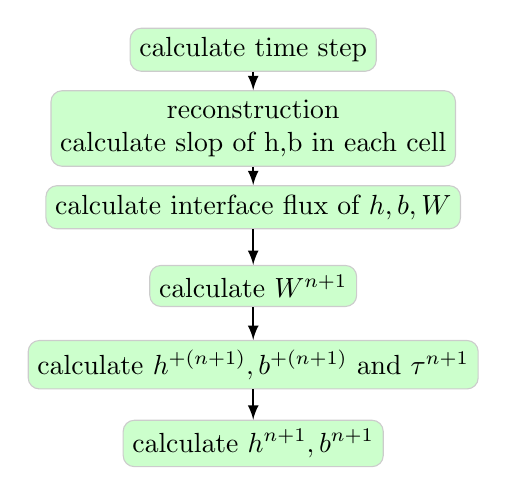
\begin{tikzpicture}[thick]
        \path[line] node[block] (time) {calculate time step};
        \path[line] node[block,below of=time] (interp) {reconstruction \\ calculate slop of h,b in each cell}
        (time) edge (interp);
        \path[line] node[block,below of=interp] (flux) {calculate interface flux of $h,b, W$}
        (interp) edge (flux);
        \path[line] node[block,below of=flux] (new-w) {calculate $W^{n+1}$}
        (flux) edge(new-w);
        \path[line] node[block,below of=new-w] (new-g) {calculate $h^{+(n+1)}, b^{+(n+1)}$ and $\tau^{n+1}$}
        (new-w) edge (new-g);
        \path[line] node[block,below of=new-g] (new-f) {calculate $h^{n+1}, b^{n+1}$}
        (new-g) edge (new-f);
    \end{tikzpicture}
    \caption{solution algorithm in one iteration}
    \label{pic:solution}
\end{figure}

\section{Nondimensionalization}
In the program, the following nondimensionalization is used,
\begin{gather*}
    \hat t=\frac{t}{t_\infty},\ \hat u_x=\frac{u_x}{C_\infty},\ \hat x=\frac{x}{L_\infty},\ \hat \rho=\frac{\rho}{\rho_\infty},\ \hat T=\frac{T}{T_\infty}, \hat p=\frac{p}{\rho_\infty C_\infty^2} \\
    \hat q=\frac{q}{\rho_\infty C_\infty^3},\ \hat h=\frac{h}{\rho_\infty/C_\infty},\ \hat b=\frac{b}{\rho_\infty},\ \hat E=\frac{E}{C_\infty^2}, \hat\mu = \frac{\mu}{\rho_\infty C_\infty L_\infty}
\end{gather*}

The free stream variables are related through
$$C_\infty=\sqrt{2RT_\infty},\ t_\infty=\frac{L_\infty}{C_\infty},\ \lambda_\infty=1/C_\infty^2$$

In the following, all variables are nondimensionalized, but we will drop the \textasciicircum for simplicity. After nondimensionalization and using the reduced distribution function, the expressions for macroscopic variables become
\begin{equation} 
    \label{eq:conserved_var}
    \begin{aligned}
        &\rho=\int h{\rm du}=\sum\alpha_k h_k\\
        &\rho U=\int hu{\rm du}=\sum\alpha_k h_k u_k\\
        &\rho E=\frac{1}{2}\left(\int hu^2{\rm du}+\int b{\rm du}\right)=\frac{1}{2}\left(\sum\alpha_k h_k u_k^2+\sum\alpha_k b_k\right)
    \end{aligned}
\end{equation}
\begin{equation} 
    \frac{K+1}{2}p=\int(u-U)^2h{\rm du}+\int b{\rm du}=\sum\alpha_k(u_k-U)^2 h_k+\sum\alpha_k b_k
\end{equation}
\begin{equation} 
    \label{eq:heatflux}
    \begin{aligned}
        q&=\frac{1}{2}\left[\int(u-U)(u-U)^2h{\rm du}+\int(u-U)b{\rm du}\right]\\
         &=\frac{1}{2}\left[\sum\alpha_k (u_k-U)(u_k-U)^2 h_k+\sum\alpha_k (u_k-U)b_k\right]
    \end{aligned}
\end{equation}
where $\alpha_k$ is the weight of the numerical integration at the k-th particle velocity. The summation is over all the discrete particle velocity.

The equation of state
\begin{equation} 
    \label{eq:eos}
    p=\frac{1}{2}\rho T,\quad \lambda=\frac{1}{T}
\end{equation}

Other expressions are not changed.

\section{Time step and reconstruction}
The time step is determined by the CFL condition
\begin{equation} 
    \Delta t={\rm CFL}\frac{\Delta x}{|U|+c}
\end{equation}
where CFL is the CFL number, $c$ is the speed of sound. The macroscopic velocity $U$ can also be replace by $\max(U,u)$

In the program, the van Leer limiter is used for the reconstruction. For example, the slope of $h$ at the i-th cell and k-th particle velocity is
\begin{equation} 
    \sigma_{i,k}^h = ({\rm sign}(s_1)+{\rm sign}(s_2))\frac{|s_1||s_2|}{|s_1|+|s_2|}
\end{equation}
where $s_1=(h_{i,k}-h_{i-1,k})/(x_i-x_{i-1}), s_2=(h_{i+1,k}-h_{i,k})/(x_{i+1}-x_{i})$.

The slope of $b$ is calculated in the same way.

\section{Calculation of interface flux}
\label{sec:inner_flux}
Take the interface $x_{i+1/2}=0$ at $t^n=0$ as example.

\subsection{The algorithm}
Here the original distribution function is used for illustration. From Eq. \ref{eq:csolution}, the integral solution at the cell interface is
\begin{equation}
    \label{eq:csolution_interface}
    f(0,t,u_k,\xi)=\frac{1}{\tau}\int_{0}^t f^+(x',t',u_k,\xi)e^{-(t-t')/\tau}dt'+e^{-t/\tau}f_0(-u_kt,0,u_k,\xi)
\end{equation}

The initial distribution function around the interface $f_0$ is
\begin{equation}
    \label{eq:f0}
    f_0(x,0,u_k,\xi) = 
    \begin{cases}
        f_{i+1/2,k}^L+\sigma_{i,k}x,& x\leqslant 0\\ 
        f_{i+1/2,k}^R+\sigma_{i+1,k}x,& x> 0\\ 
    \end{cases}
\end{equation}
where $f_{i+1/2,k}^L, f_{i+1/2,k}^R$ are the reconstructed initial distribution functions at the left and right side of the interface.

The Maxwellian distribution around the interface in $f^+$ is approximated by Taylor expansion
\begin{equation} 
    \label{eq:g_interface}
    g(x,t,u,\xi)=g_0[1+(1-H[x])a^Lx+H[x]a^Rx+At]
\end{equation}
where $g_0$ is the Maxwellian distribution at $x=0,t=0$ and $H[x]$ is the Heaviside function$$H[x]=\begin{cases}0,& x<0\\ 1,& x\geqslant 0\end{cases}$$

$a^L,a^R$ and $A$ have the same form,
$$ a = a_1+a_2u+a_3\frac{1}{2}(u^2+\xi^2)$$
where $a_1,a_2,a_3$ are local constants

Inserting Eq. \ref{eq:f0} and Eq. \ref{eq:g_interface} into Eq. \ref{eq:csolution_interface}, one obtains
\begin{equation} 
    \label{eq:csolution_final}
    \begin{aligned}
        f(0,t,u_k,\xi)=&(1-e^{-t/\tau})(g_0+g^+)\\
                       &+(\tau(-1+e^{-t/\tau})+te^{-t/\tau})(a^LH[u_k]+a^R(1-H[u_k]))u_kg_0\\
                       &+\tau(t/\tau-1+e^{-t/\tau})Ag_0\\
                       &+e^{-t/\tau}((f_{i+1/2,k}^L-u_kt\sigma_{i,k})H[u_k]+(f_{i+1/2,k}^R-u_kt\sigma_{i+1,k})(1-H[u_k]))\\
        =&{\tilde g}_{i+1/2,k}+{\tilde f}_{i+1/2,k}
    \end{aligned}
\end{equation}
where ${\tilde g}_{i+1/2,k}$ is the first three terms related to equilibrium distribution, ${\tilde f}_{i+1/2,k}$ is the last two terms related to the initial non-equilibrium distribution

$g_0$ or $W_0$ can be obtained by applying the capability condition at $x=0,t=0$
$$\int (f^+-f)|_{x=0,t=0}\psi d\Xi=0$$
which gives
\begin{equation} 
    \label{eq:solve_g0}
    W_0=\int g_0\psi d\Xi=\int f_0(0,0,u_k,\xi)\psi d\Xi
\end{equation}

$a^L,a^R,A$ are obtained from the slope of conservative variables
\begin{equation}
    \label{eq:microslope_space}
    \frac{1}{\rho_0}\left(\frac{\partial W}{\partial x}\right)^L=\int a^L g_0\psi d\Xi,\quad \frac{1}{\rho_0}\left(\frac{\partial W}{\partial x}\right)^R=\int a^R g_0\psi d\Xi
\end{equation}
\begin{equation} 
    \label{eq:microslope_time}
    \frac{1}{\rho_0}\frac{\partial W}{\partial t}=\int Ag_0\psi d\Xi
\end{equation}

The time derivative of $W$ can be calculated via the capability condition
$$\left.\frac{\rm d}{{\rm d}t}\int(f^+-f)\psi d\Xi\right|_{x=0,t=0}=0$$
which gives
\begin{equation} 
    \label{eq:solve_wt}
    \frac{\partial W}{\partial t} = -\int\left(a^LH[u]+a^R(1-H[u])\right)ug_0\psi d\Xi
\end{equation}

\subsection{The numerical procedure}
The flow chart of the numerical procedure is shown in Figure. \ref{pic:flux}

\begin{figure}[htb!]
    \centering
    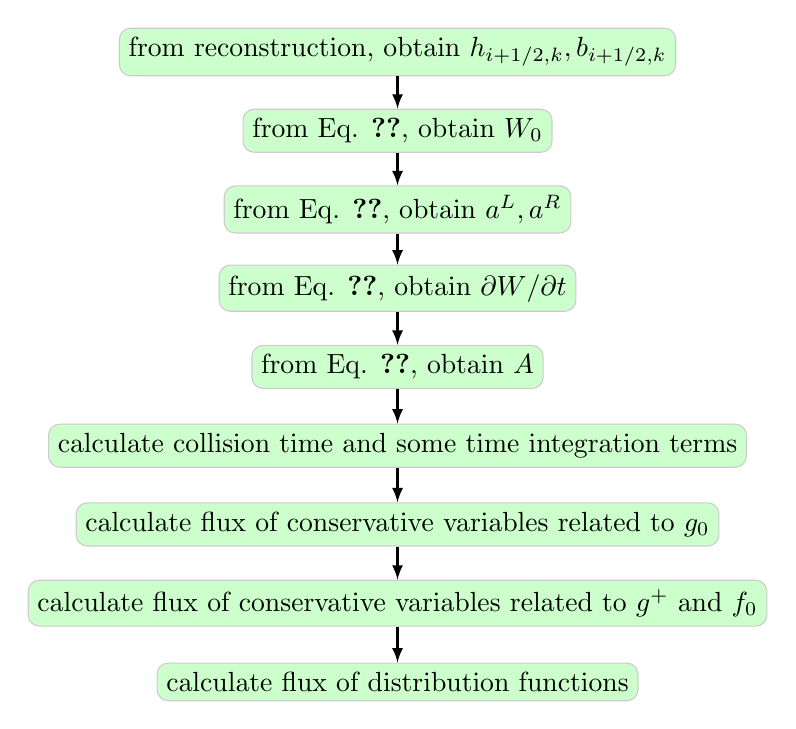
\begin{tikzpicture}[thick]
        \path[line] node[block] (f0) {from reconstruction, obtain $h_{i+1/2,k},b_{i+1/2,k}$};
        \path[line] node[block,below of=f0] (w0) {from Eq. \ref{eq:solve_g0}, obtain $W_0$}
        (f0) edge (w0);
        \path[line] node[block,below of=w0] (as) {from Eq. \ref{eq:microslope_space}, obtain $a^L,a^R$}
        (w0) edge (as);
        \path[line] node[block,below of=as] (wt) {from Eq. \ref{eq:solve_wt}, obtain ${\partial W}/{\partial t}$}
        (as) edge (wt);
        \path[line] node[block,below of=wt] (at) {from Eq. \ref{eq:microslope_time}, obtain $A$}
        (wt) edge (at);
        \path[line] node[block,below of=at] (tt) {calculate collision time and some time integration terms}
        (at) edge (tt);
        \path[line] node[block,below of=tt] (gg) {calculate flux of conservative variables related to $g_0$}
        (tt) edge (gg);
        \path[line] node[block,below of=gg] (gf) {calculate flux of conservative variables related to $g^+$ and $f_0$}
        (gg) edge (gf);
        \path[line] node[block,below of=gf] (ff) {calculate flux of distribution functions}
        (gf) edge (ff);
    \end{tikzpicture}
    \caption{interface flux calculation}
    \label{pic:flux}
\end{figure}

\subsubsection*{Reconstruct initial distribution}
Take $h$ as example. Since we take value from $h_{i+1/2,k}^L$ only if $u_k\geqslant 0$ and take value from $h_{i+1/2,k}^R$ only if $u_k <0$ (see Eq. \ref{eq:csolution_final}), there is no need to store the left and right values separately. 

Instead, we define the variable
$$h_{i+1/2,k} = \begin{cases} h_{i,k}+(x_{i+1/2}-x_i)\sigma_{i,k}^h, & u_k \geqslant 0\\ h_{i+1,k}-(x_{i+1}-x_{i+1/2})\sigma_{i+1,k}^h, & u_k < 0\end{cases}
$$
and similarly
$$
\sigma_{i+1/2,k}^h = \begin{cases} \sigma_{i,k}^h, & u_k \geqslant 0\\ \sigma_{i+1,k}^h, & u_k < 0\end{cases}
$$

In the program, they are written as
$$h_{i+1/2,k} =\sigma_{i,k}^h H[u_k]+\sigma_{i+1,k}^h(1-H[u_k])$$
and
$$\sigma_{i+1/2,k}^h = (h_{i,k}+(x_{i+1/2}-x_i)\sigma_{i,k}^h)H[u_k]+(h_{i+1,k}-(x_{i+1}-x_{i+1/2})\sigma_{i+1,k}^h)(1-H[u_k])$$

\subsubsection*{Calculate $W_0$}
$W_0$ is calculated from Eq. \ref{eq:conserved_var}, with $h_k=h_{i+1/2,k}, b_k=b_{i+1/2,k}$

Then the primary variables is obtained from the relation(the expression for $\lambda$ only holds for equilibrium state)
$$\rho_0 = \rho_0,\quad U_0=\frac{\rho_0 U_0}{\rho_0},\quad \lambda_0=\frac{(K+1)\rho_0}{4\left(\rho_0 E_0-\frac{1}{2}\rho(U_0^2+V_0^2)\right)}$$

The heat flux is calculated by Eq. \ref{eq:heatflux}, with $h_k=h_{i+1/2,k},b_k=b_{i+1/2,k},U=U_0$

\subsubsection*{Calculate $a^L,a^R$}
The macroscopic slope is approximated by
$$\left(\frac{\partial W}{\partial x}\right)^L\approx\frac{W_0-W_{i}}{x_{i+1/2}-x_i},\quad \left(\frac{\partial W}{\partial x}\right)^R\approx\frac{W_{i+1}-W_{0}}{x_{i+1}-x_{i+1/2}}$$
and the three components of $a^L,a^R$ are calculated from
\begin{equation} 
    \label{eq:micro_slope}
    \begin{aligned}
        a_3&=\frac{4\lambda_0^2}{(K+1)\rho_0}\left[2\frac{\partial\rho E}{\partial x}+\left(U_0^2-\frac{K+1}{2\lambda_0}\right)\frac{\partial\rho}{\partial x}-2U_0\frac{\partial\rho U}{\partial x}\right]\\
        a_2&=\frac{2\lambda_0}{\rho_0}\left(\frac{\partial\rho U}{\partial x}-U_0\frac{\partial\rho}{\partial x}\right)-U_0a_3\\
        a_1&=\frac{1}{\rho_0}\frac{\partial\rho}{\partial x}-U_0a_2-\frac{1}{2}\left(U_0^2+\frac{K+1}{2\lambda_0}\right)a_3
    \end{aligned}
\end{equation}

\subsubsection*{Calculate ${\partial W}/{\partial t}$ and $A$}
From Eq. \ref{eq:solve_wt}, the time derivative of $W$ is calculated from
$$\frac{\partial W}{\partial t}=-\rho_0\left(<a^Lu\psi>_{>0}+<a^Ru\psi>_{<0}\right)$$
where $<...>$ is the moments of Maxwellian distribution function. The detail definition and calculation can be found in \nameref{appendix:moments}

$A$ is calculated in the same way as $a^L,a^R$ using Eq. \ref{eq:micro_slope}.

\subsubsection*{Calculate collision time and some time integration terms}
From Eq. \ref{eq:viscosity} and Eq. \ref{eq:eos}, the collision time is
$$\tau = \frac{2\lambda_0^{1-\omega}}{\rho_0}\mu_{\infty}$$

Some time integrals used in the evaluation of flux is listed below
$$
\begin{aligned}
    Mt_4 &= \int_{t^n}^{t^{n+1}} e^{-t/\tau}dt = \tau(1-e^{-\Delta t/\tau}) \\
    Mt_5 &= \int_{t^n}^{t^{n+1}} te^{-t/\tau}dt = -\tau\Delta t e^{-\Delta t/\tau}+\tau Mt_4 \\
    Mt_1 &= \int_{t^n}^{t^{n+1}} (1-e^{-t/\tau})dt = \Delta t-Mt_4 \\
    Mt_2 &= \int_{t^n}^{t^{n+1}} (\tau(-1+e^{-t/\tau})+te^{-t/\tau})dt = -\tau Mt_1+Mt_5 \\
    Mt_3 &= \int_{t^n}^{t^{n+1}} \tau(t/\tau-1+e^{-t/\tau})dt = \frac{1}{2}\Delta t^2-\tau Mt_1
\end{aligned} 
$$

\subsubsection*{Calculate the flux of conservative variables related to $g_0$}
Theoretically, $\int_{t^n}^{t^{n+1}}\int {\tilde g}_{i+1/2}u\psi d\Xi dt$ can be calculated analytically. But the integration related to $g^+$ is too complex, and will be calculated with numerical integration. Only the terms related to $g_0$ will be integrated analytically here.
$${\bf W}_{g_0} = Mt_1\rho_0<u\psi>+Mt_2\rho_0\left(<a^Lu^2\psi>_{>0}+<a^Ru^2\psi>_{<0}\right)+Mt_3\rho_0<Au\psi>$$

\subsubsection*{Calculate the flux of conservative variables related to $g^+$ and $f_0$}
First evaluate $H_k,B_k$ corresponding to $g_0$ by Eq. \ref{eq:reduced_g},
$$H_k = \rho_0\left(\frac{\lambda_0}{\pi}\right)^{1/2}e^{-\lambda_0(u_k-U_0)^2},\quad B_k = \frac{K}{2\lambda_0}H_k$$
and then evaluate $H_{k}^+,B_{k}^+$ corresponding to $g^+$ by Eq. \ref{eq:reduced_gp}
$$
\begin{aligned}
    & H_k^+ = \frac{4(1-\Pr)\lambda_0^2}{5\rho_0}(u_k-U_0)q(2\lambda_0(u_k-U_0)^2+k-5)H_k\\
    & B_k^+ = \frac{4(1-\Pr)\lambda_0^2}{5\rho_0}(u_k-U_0)q(2\lambda_0(u_k-U_0)^2+k-3)B_k
\end{aligned}
$$
The flux of conservative variables related to $g^+$ is,
$$
{\bf W}_{g^+} = Mt_1
\begin{pmatrix}
    \sum\alpha_k u_k H_k^+\\ \sum\alpha_k u_k^2 H_k^+\\ \frac{1}{2}\left(\sum\alpha_k u_k^3 H_k^+ + \sum\alpha_k u_k B_k^+\right)
\end{pmatrix}
$$

The flux of conservative variables related to $f_0$ is,
$$
{\bf W}_{f_0} = Mt_4
\begin{pmatrix}
    \sum\alpha_k u_k h_{i+1/2,k}\\ \sum\alpha_k u_k^2 h_{i+1/2,k}\\ \frac{1}{2}\left(\sum\alpha_k u_k^3 h_{i+1/2,k}+\sum\alpha_k u_k b_{i+1/2,k}\right)
\end{pmatrix}
-Mt_5
\begin{pmatrix}
    \sum\alpha_k u_k^2 \sigma_{i+1/2,k}^h\\ \sum\alpha_k u_k^3 \sigma_{i+1/2,k}^h\\ \frac{1}{2}\left(\sum\alpha_k u_k^4 \sigma_{i+1/2,k}^h+\sum\alpha_k u_k^2 \sigma_{i+1/2,k}^b\right)
\end{pmatrix}
$$

The flux of conservative variables is
$${\bf W}_{i+1/2} = \int_{t^n}^{t^{n+1}}\int f_{i+1/2}u\psi d\Xi dt={\bf W}_{g_0}+{\bf W}_{g^+}+{\bf W}_{f_0}$$

\subsubsection*{Calculate the flux of distribution functions}
The flux of reduced distribution function $h$ is calculated by
$$
\begin{aligned}
    {\bf F}_{i+1/2,k}^h &= \int_{t^n}^{t^{n+1}}\int f_{i+1/2,k}u_k d\xi dt\\
                        &= Mt_1 u_k (H_k+H_k^+)\\
                        &+ Mt_2 u_k^2 \left(a_1^L H_k + a_2^L u_k H_k + \frac{1}{2}a_3^L(u_k^2 H_k+B_k)\right)H[u_k]\\
                        &+ Mt_2 u_k^2 \left(a_1^R H_k + a_2^R u_k H_k + \frac{1}{2}a_3^R(u_k^2 H_k+B_k)\right)(1-H[u_k])\\
                        &+ Mt_3 u_k \left(A_1 H_k + A_2 u_k H_k + \frac{1}{2}A_3(u_k^2 H_k+B_k)\right)\\
                        &+ Mt_4 u_k h_{i+1/2,k}-Mt_5 u_k^2 \sigma_{i+1/2,k}^h
\end{aligned} 
$$

The flux of reduced distribution function $b$ is calculated by
$$
\begin{aligned}
    {\bf F}_{i+1/2,k}^h &= \int_{t^n}^{t^{n+1}}\int f_{i+1/2,k}u_k d\xi dt\\
                        &= Mt_1 u_k (B_k+B_k^+)\\
                        &+ Mt_2 u_k^2 \left(a_1^L B_k + a_2^L u_k B_k + \frac{1}{2}a_3^L(u_k^2 B_k+<\xi^4>H_k)\right)H[u_k]\\
                        &+ Mt_2 u_k^2 \left(a_1^R B_k + a_2^R u_k B_k + \frac{1}{2}a_3^R(u_k^2 B_k+<\xi^4>H_k)\right)(1-H[u_k])\\
                        &+ Mt_3 u_k \left(A_1 B_k + A_2 u_k B_k + \frac{1}{2}A_3(u_k^2 B_k+<\xi^4>H_k)\right)\\
                        &+ Mt_4 u_k b_{i+1/2,k}-Mt_5 u_k^2 \sigma_{i+1/2,k}^b
\end{aligned} 
$$

\section{Update cell averaged value}
The procedure is shown in Figure. \ref{pic:update}

\begin{figure}[htb!]
    \centering
    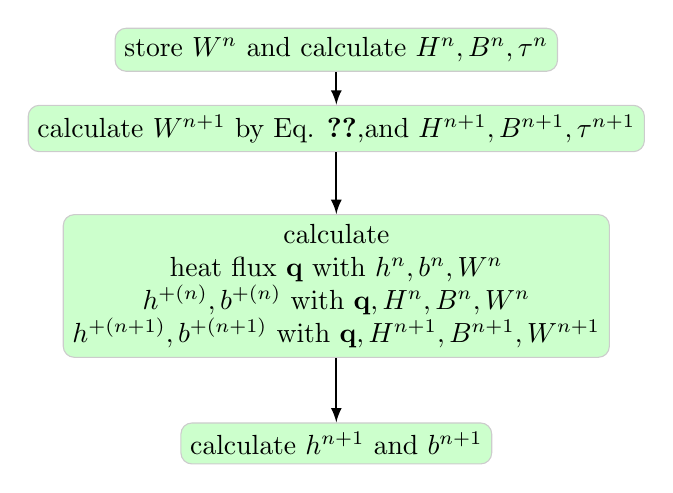
\begin{tikzpicture}[thick]
        \path[line] node[block] (wn) {store $W^n$ and calculate $H^n,B^n,\tau^n$};
        \path[line] node[block,below of=wn] (ww) {calculate $W^{n+1}$ by Eq. \ref{eq:conservative_discrete},and $H^{n+1},B^{n+1},\tau^{n+1}$}
        (wn) edge (ww);
        \path[line] (ww) ++(0,-2.0) coordinate node[block] (gp) {calculate\\heat flux ${\bf q}$ with $h^n,b^n,W^n$\\ $h^{+(n)},b^{+(n)}$ with ${\bf q},H^n,B^n,W^n$\\ $h^{+(n+1)},b^{+(n+1)}$ with ${\bf q},H^{n+1},B^{n+1},W^{n+1}$}
        (ww) edge (gp);
        \path[line] (gp) ++(0,-2.0) coordinate node[block] (ff) {calculate $h^{n+1}$ and $b^{n+1}$}
        (gp) edge (ff);
    \end{tikzpicture}
    \caption{update cell averaged value}
    \label{pic:update}
\end{figure}

The equation for updating $h^{n+1}$ and $b^{n+1}$ can be obtained from Eq. \ref{eq:bgk-shakhov_discrete}
$$
\begin{aligned}
    h_{i,k}^{n+1} &= \left(1+\frac{\Delta t}{2\tau^{n+1}}\right)^{-1}\left[h_{i,k}^n+\frac{1}{\Delta x}({\bf F}_{i-1/2}^h-{\bf F}_{i+1/2}^h)+\frac{\Delta t}{2}\left(\frac{h_{i,k}^{+(n+1)}}{\tau^{n+1}}+\frac{h_{i,k}^{+(n)}-h_{i,k}^n}{\tau^n}\right)\right]\\
    b_{i,k}^{n+1} &= \left(1+\frac{\Delta t}{2\tau^{n+1}}\right)^{-1}\left[b_{i,k}^n+\frac{1}{\Delta x}({\bf F}_{i-1/2}^b-{\bf F}_{i+1/2}^b)+\frac{\Delta t}{2}\left(\frac{b_{i,k}^{+(n+1)}}{\tau^{n+1}}+\frac{b_{i,k}^{+(n)}-b_{i,k}^n}{\tau^n}\right)\right]\\
\end{aligned} 
$$

\section{Boundary condition}
Only isothermal wall boundary condition with complete accommodation is discussed. Assuming left wall($x=1/2$). The boundary condition described here is quiet simple, the incoming distribution function is directly obtained through interpolation. One can also use the same method as the inner region to calculate the incoming distribution and flux.

First, obtain $h_k^{in},b_k^{in}$ by one-sided interpolation from the interior region. For example,
$$h_{k}^{in} = h_{1,k}-\sigma_{1,k}^h\frac{\Delta x}{2}$$

Second, calculate the density at the wall with the condition that no particle penetrating the wall
$$\int_{t^n}^{t^{n+1}}\int_{u>0} ug_w d\Xi dt+\int_{t^n}^{t^{n+1}}\int_{u<0} uf^{in}d\Xi dt=0$$
which gives
$$\rho_w = -\frac{\sum\alpha_k u_k h_k^{in}}{\left(\frac{\lambda_w}{\pi}\right)^{1/2}\sum\alpha_k u_k e^{-\lambda_w(u_k-U_w)^2}}$$
where $g_w,\rho_w,\lambda_w,U_w$ are the variables at the wall.

The corresponding reduced Maxwellian distribution at the wall $H_k^w,B_k^w$ is also obtained.

Thirdly, the distribution function at the boundary interface is expressed by (same holds for $b_k$)
$$h_k = H_k^wH[u_k]+h_k^{in}(1-H[u_k])$$

Finally, the flux across the wall is calculated by
$$
{\bf W}_{1/2} = \Delta t
\begin{pmatrix}
    \sum\alpha_k u_k h_k\\
    \sum\alpha_k u_k^2 h_k\\
    \sum\alpha_k \frac{1}{2}\left(u_k^3 h_k+u_k b_k\right)
\end{pmatrix} 
$$
and
$$
\begin{aligned}
    {\bf F}_{1/2,k}^h &= \Delta t u_k h_k\\
    {\bf F}_{1/2,k}^b &= \Delta t u_k b_k
\end{aligned} 
$$

%code
\chapter{UGKS Code}
\section{Usage}
\subsection{Compiling}
A makefile is provided to compile the program under Linux. If you are using any IDE (e.g. Visual Studio), use the compiling function provided by the IDE.

The makefile can be used to compile the two codes, UGKS1D and UGKS2D, and also this manual. There are several requirements for the makefile to work.
\begin{itemize}
    \item Fortran Compiler: either \hi{ifort} or \hi{gfortran}, supporting Fortran 2003
    \item Bash shell
    \item Latex: only for compilation of the manual. It requires \hi{hyperref}, \hi{parskip}, \hi{amsmath}, \hi{amssymb}, \hi{fullpage}, \hi{appendix}, \hi{graphicx}, \hi{subfigure}, \hi{xcolor}, \hi{listings} or \hi{minted} packages, and also \hi{bibtex}, \hi{dvips} and \hi{ps2pdf}.
\end{itemize}

By default, the make command will compile both UGKS1D and UGKS2D with openmp and ifort. This behavior can be changed by specifying the target and passing parameters.

\begin{enumerate}
    \item Compile both UGKS1D and UGKS2D with openmp and ifort  
        \begin{minted}[gobble=8]{sh}
            make
        \end{minted}
    \item Only compile UGKS1D
        \begin{minted}[gobble=8]{sh}
            make 1D
        \end{minted}
    \item Only compile UGKS2D
        \begin{minted}[gobble=8]{sh}
            make 2D
        \end{minted}
    \item Compile both UGKS1D and UGKS2D, but \textbf{WITHOUT} openmp, and \textbf{WITH} gfortran
        \begin{minted}[gobble=8]{sh}
            make OMP=no FC=gfortran
        \end{minted}
    \item Compile the manual
        \begin{minted}[gobble=8]{sh}
            make manual
        \end{minted}
    \item Clean the compilation
        \begin{minted}[gobble=8]{sh}
            make clean
        \end{minted}
\end{enumerate}

The executables will be put into the bin directory, and the compiled manual.pdf will in the doc directory.

\subsection{Running}
Just type the program name to run it under the bin directory, no input file or data is required. 

The code will generate two files,
\begin{itemize}
    \item *.hst : record the convergence history every 10 iterations.
    \item *.rst : record the final result of the program.
\end{itemize}
Both files are in tecplot format and will be put into current working directory.

\subsection{Other information}
The comments in the program are written in doxygen format, and can be used to generate documentation of the code. But the doxygen configuration file is not included, and the documentation generation is not tested.

This program uses \href{http://git-scm.com/}{GIT} for version control, and the source repository is published on \href{https://github.com/lainme/UGKS}{GitHub}. To obtain the code via git, use the following command,

\begin{minted}{sh}
    git clone git://github.com/lainme/UGKS.git
\end{minted}

\section{UGKS1D Code}
Once the flow condition before the normal shock is known (upstream), the flow variables after the shock (downstream) can be calculated by normal shock relation,
\begin{equation}
    \label{eq:normal_shock}
    \begin{aligned}
        M_2 &= \sqrt{\frac{M_1^2(\gamma-1)+2}{2\gamma M_1^2-(\gamma-1)}}\\
        \frac{\rho_2}{\rho_1} &= \frac{(\gamma+1)M_1^2}{(\gamma-1)M_1^2+2}\\
        \frac{T_2}{T_1} &= \frac{(1+\frac{\gamma-1}{2}M_1^2)(\frac{2\gamma}{\gamma-1}M_1^2-1)}{M_1^2(\frac{2\gamma}{\gamma-1}+\frac{\gamma-1}{2})}
    \end{aligned}
\end{equation}
where $M_1,\rho_1,T_1$ are upstream Mach number, density and temperature. $M_2,\rho_2,T_2$ are downstream Mach number, density and temperature.

For shock structure calculation, the upstream and downstream conditions are specified at the two boundaries (via ghost cell). And the flux across the interfaces are calculated through the same method described in section \ref{sec:inner_flux}.

In the UGKS1D code, the reference state is,
$$L_\infty=l_{mfp,1},\quad T_\infty=T_1,\quad \rho_\infty = \rho_1$$
where $l_{mfp,1}$ is the upstream mean free path.

There are several important options in the code,
\begin{itemize}
    \item \textbf{method\_output}: the method to output the solution. If set to \hi{ORIGINAL}, the original nondimensionalized values will be written to the result file. If set to \hi{NORMALIZE}, the density will be normalized by $\rho = (\rho-\rho_1)/(\rho_2-\rho_1)$ and the temperature is also normalized by the same way
    \item \textbf{mu\_ref}: the reference viscosity coefficient $\mu_\infty$. Can be specified directly or calculated through the provided function \hi{get\_mu}. This function calculate the viscosity coefficient through
        $$\mu_\infty = \frac{5(\alpha+1)(\alpha+2)\sqrt{\pi}}{4\alpha(5-2\omega)(7-2\omega)}{\rm Kn}_\infty$$
        where $\alpha,\omega$ are coefficients related to molecule model. 
\end{itemize}

The default settings in the code is for Argon shock structure calculation at ${\rm Ma}=8.0$, see \cite{Xu2011}
\begin{itemize}
    \item Argon gas with Prandlt number $\Pr=2.0/3.0$ and variable hard-sphere model $\omega=0.72$
    \item Mach number 8.0
    \item Newton-Cotes integration with 100 velocity points ranges from -15 to 15.
    \item Computation domain is 50 times of the upstream mean free path
    \item Cell size is half of the upstream mean free path
    \item Output solution at $t=250$
\end{itemize}

Figure. \ref{pic:shock_solution} shows the comparison of the simulated density with the experimental measurements \cite{Alsmeyer1976} and also temperature profile .

\begin{figure}[htb!]
    \centering
    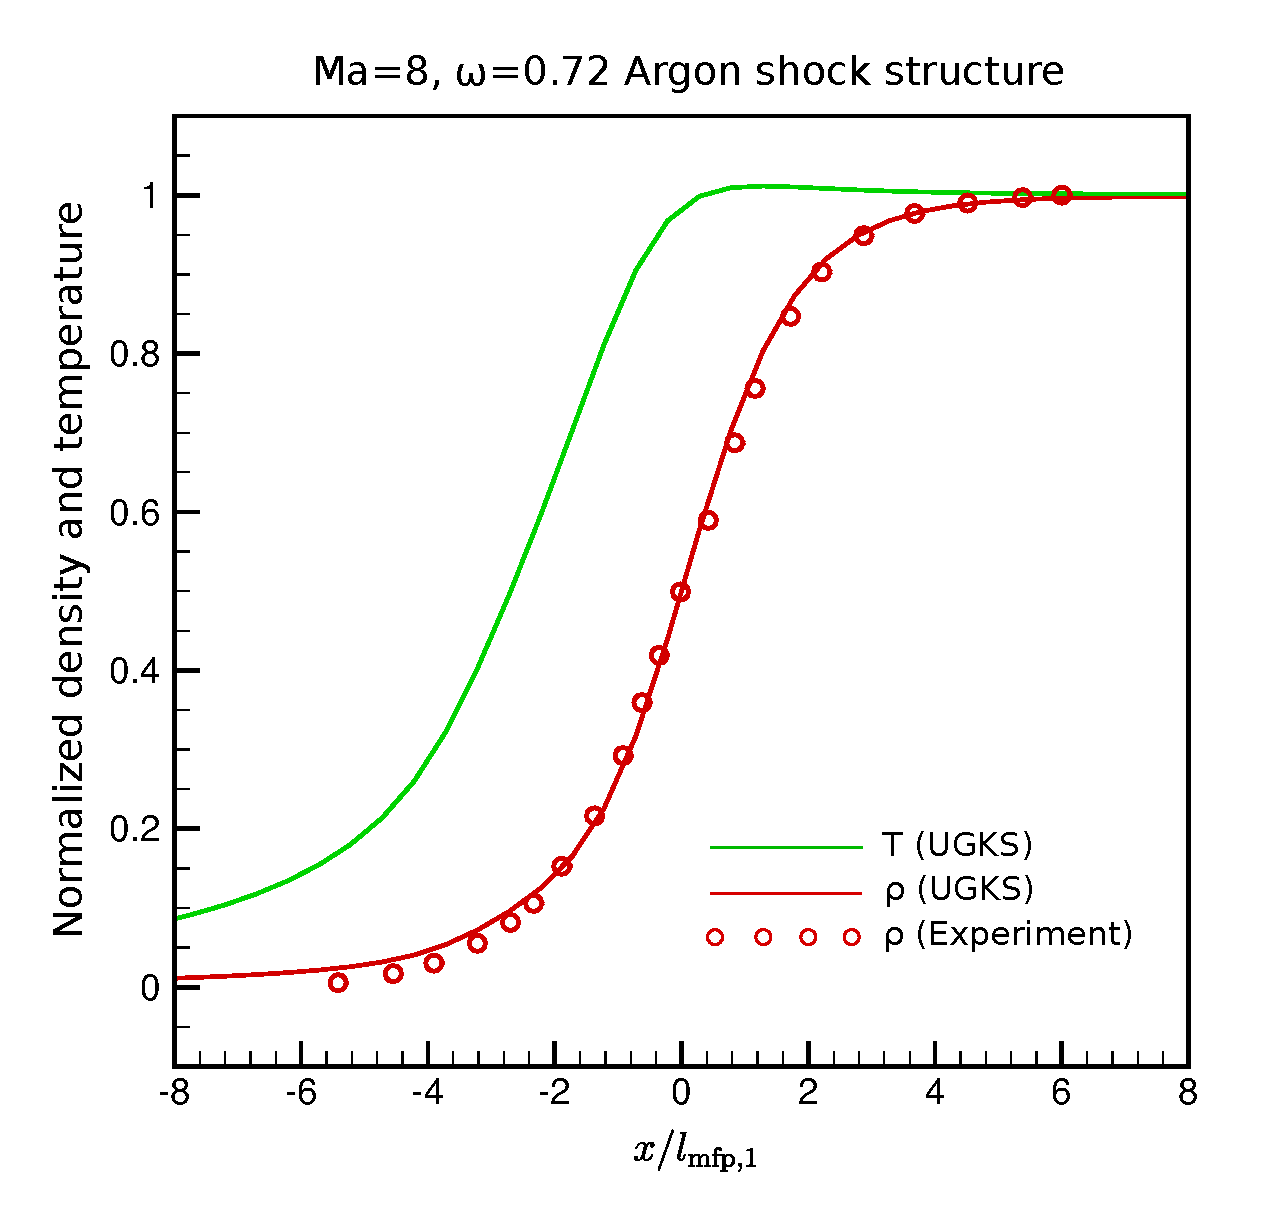
\includegraphics[width=7cm,height=6.5cm]{shock_Ma8.eps}
    \caption{Argon shock structure at ${\rm Ma}=8.0$.}
    \label{pic:shock_solution}
\end{figure}

\section{UGKS2D Code}
\subsection{Differences with 1D}
For 2D problem, many expressions need to be slightly changed. For example,
$$g=\rho\left(\frac{\lambda}{\pi}\right)^{\frac{K+2}{2}}e^{-\lambda((u-U)^2+(v-V)^2+\xi^2)}$$
where $v$ is particle velocity in y direction, $V$ is macroscopic velocity in y direction. 

The relation between $K$ and $\gamma$ becomes
$$\gamma=\frac{K+4}{K+2}$$

The reduced Maxwellian distribution becomes ($B$ is not changed)
$$H=\int_{-\infty}^{\infty}gd\xi=\rho\left(\frac{\lambda}{\pi}\right)e^{-\lambda((u-U)^2+(v-V)^2)}$$

The collision invariants are $\psi=(1,u,v,1/2(u^2+v^2+\xi^2))^T$. And the expressions for macroscopic variables are correspondingly changed. For example, the nondimensionalized pressure is calculated via
$$\frac{K+2}{2}p=\int((u-U)^2+(v-V)^2)hdu+\int bdu$$

When calculating the flux, the slopes related to Maxwellian becomes
$$a=a_1+a_2u+a_3v+a_4\frac{1}{2}(u^2+v^2+\xi^2)$$
and the components are calculated via
$$
\begin{aligned}
    a_4&=\frac{4\lambda_0^2}{(K+2)\rho_0}\left[2\frac{\partial\rho E}{\partial x}+\left(U_0^2+V_0^2-\frac{K+2}{2\lambda_0}\right)\frac{\partial\rho}{\partial x}-2U_0\frac{\partial\rho U}{\partial x}-2V_0\frac{\partial\rho V}{\partial x}\right]\\
    a_3&=\frac{2\lambda_0}{\rho_0}\left(\frac{\partial\rho V}{\partial x}-V_0\frac{\partial\rho}{\partial x}\right)-V_0a_4\\
    a_2&=\frac{2\lambda_0}{\rho_0}\left(\frac{\partial\rho U}{\partial x}-U_0\frac{\partial\rho}{\partial x}\right)-U_0a_4\\
    a_1&=\frac{1}{\rho_0}\frac{\partial\rho}{\partial x}-U_0a_2-V_0a_3-\frac{1}{2}\left(U_0^2+V_0^2+\frac{k+2}{2\lambda_0}\right)a_4
\end{aligned}
$$

\subsection{Lid-driven cavity problem}
The test case included in UGKS2D code is Lid-driven cavity problem\cite{Huang2012}. The argon gas is enclosed by four walls to form a rectangular shape. The upper wall is moving in tangential direction with velocity $U_W$, other walls are stationary. All walls are kept at a constant temperature $T_W$, and full accommodation is assumed. The gas is initially at rest with the same temperature as the wall.  Figure. \ref{pic:cavity} shows the schematic of the problem.

\begin{figure}[htb!]
    \centering
    \begin{tikzpicture}[thick]
        \node[rectangle,draw,minimum size=5cm] (bx) {Argon};
        \node at ($(bx)+(-3,+0)$) {$T_W$};
        \node at ($(bx)+(+3,+0)$) {$T_W$};
        \node at ($(bx)+(+0,-3)$) {$T_W$};
        \node at ($(bx)+(+0,+3.2)$) {$U_W,T_W$};
        \draw[line] ($(bx)+(-1,+2.8)$) -- ($(bx)+(+1,+2.8)$);
    \end{tikzpicture}
    \caption{Schematic of Lid-driven cavity problem}
    \label{pic:cavity}
\end{figure}

In the code, the default test case is for $T_W = 273K, U_W=50m/s, {\rm Kn} = l_{mfp}/{L} = 0.075$, where $l_{mfp}$ is mean free path and $L$ is the domain length.

Choose the initial condition as reference state, the settings are
\begin{itemize}
    \item Second order interpolation
    \item VHS model for collision time and HS model for reference state
    \item Prandtl number $\Pr=2.0/3.0$, Knudsen number ${\rm Kn}_\infty=0.075$ (at reference state)
    \item $T_W=1, U_W=0.15$
    \item $L=1$ with 45x45 grids
    \item Gaussian quadrature with 28x28 velocity points
\end{itemize}

Figure. \ref{pic:cavity_solution} shows the result for the above setup, and compared with the DSMC solution\cite{John2011}.

\begin{figure}[htb!]
    \centering
    \subfigure[Temperature contour]{
        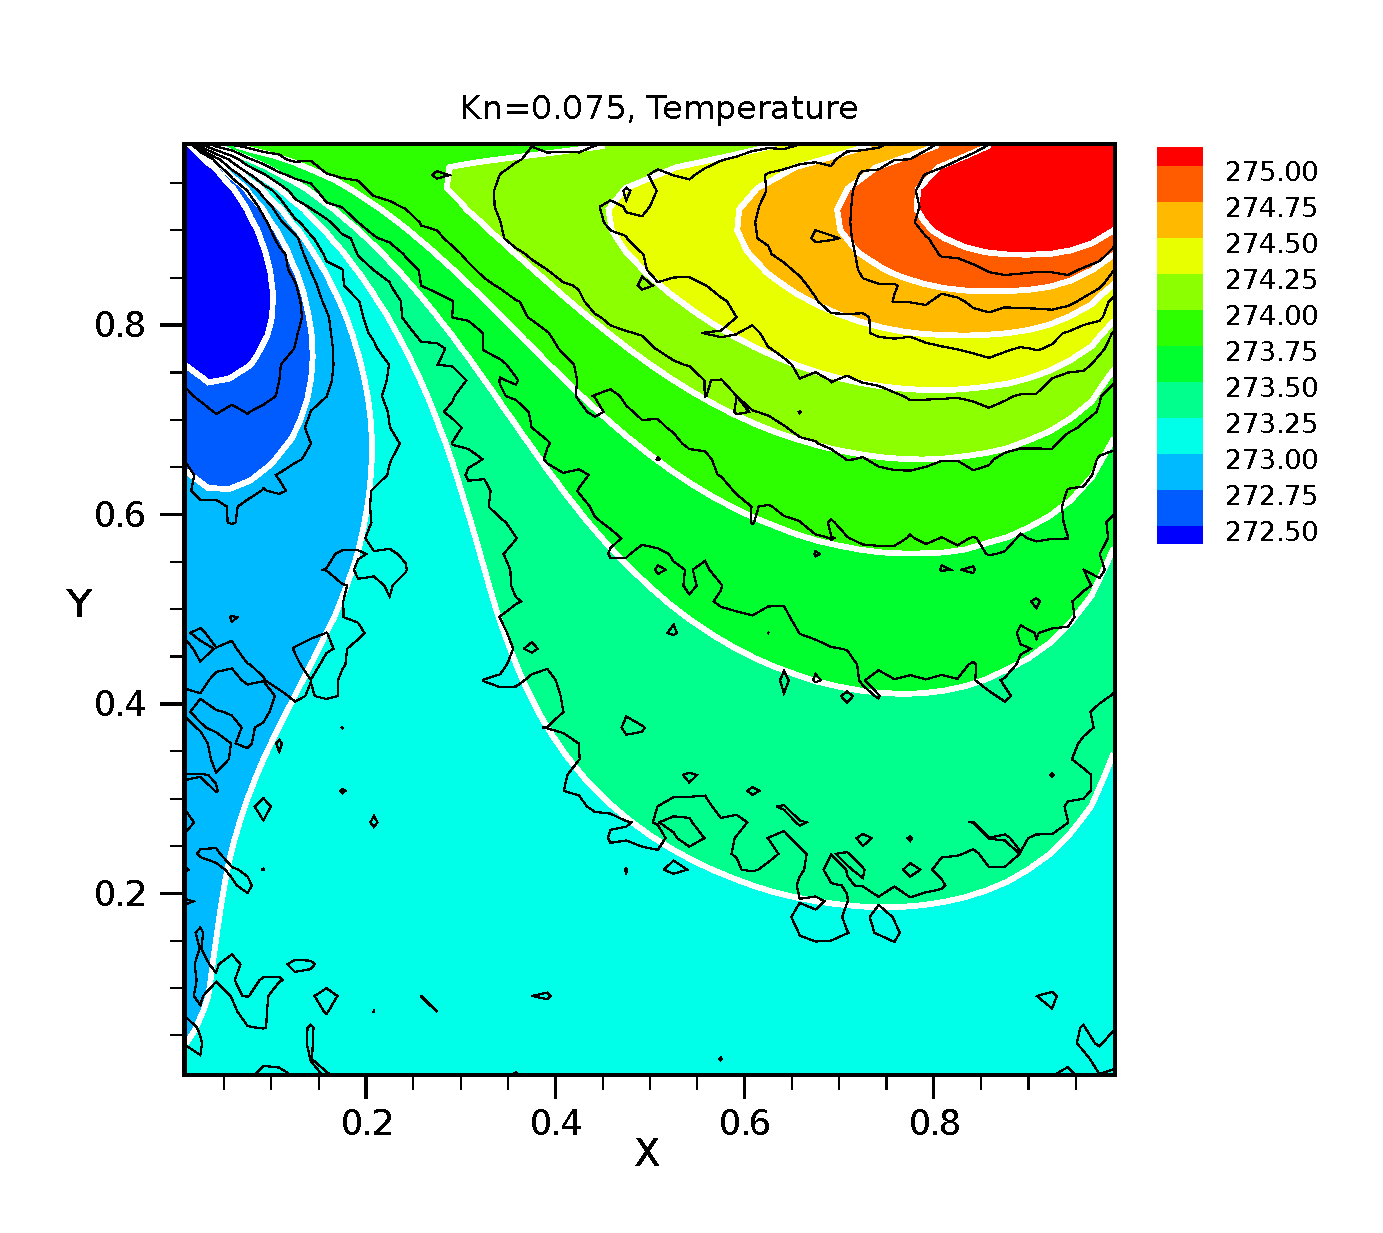
\includegraphics[width=7cm,height=6.5cm]{temperature.eps}
    }
    \subfigure[Heat flux]{
        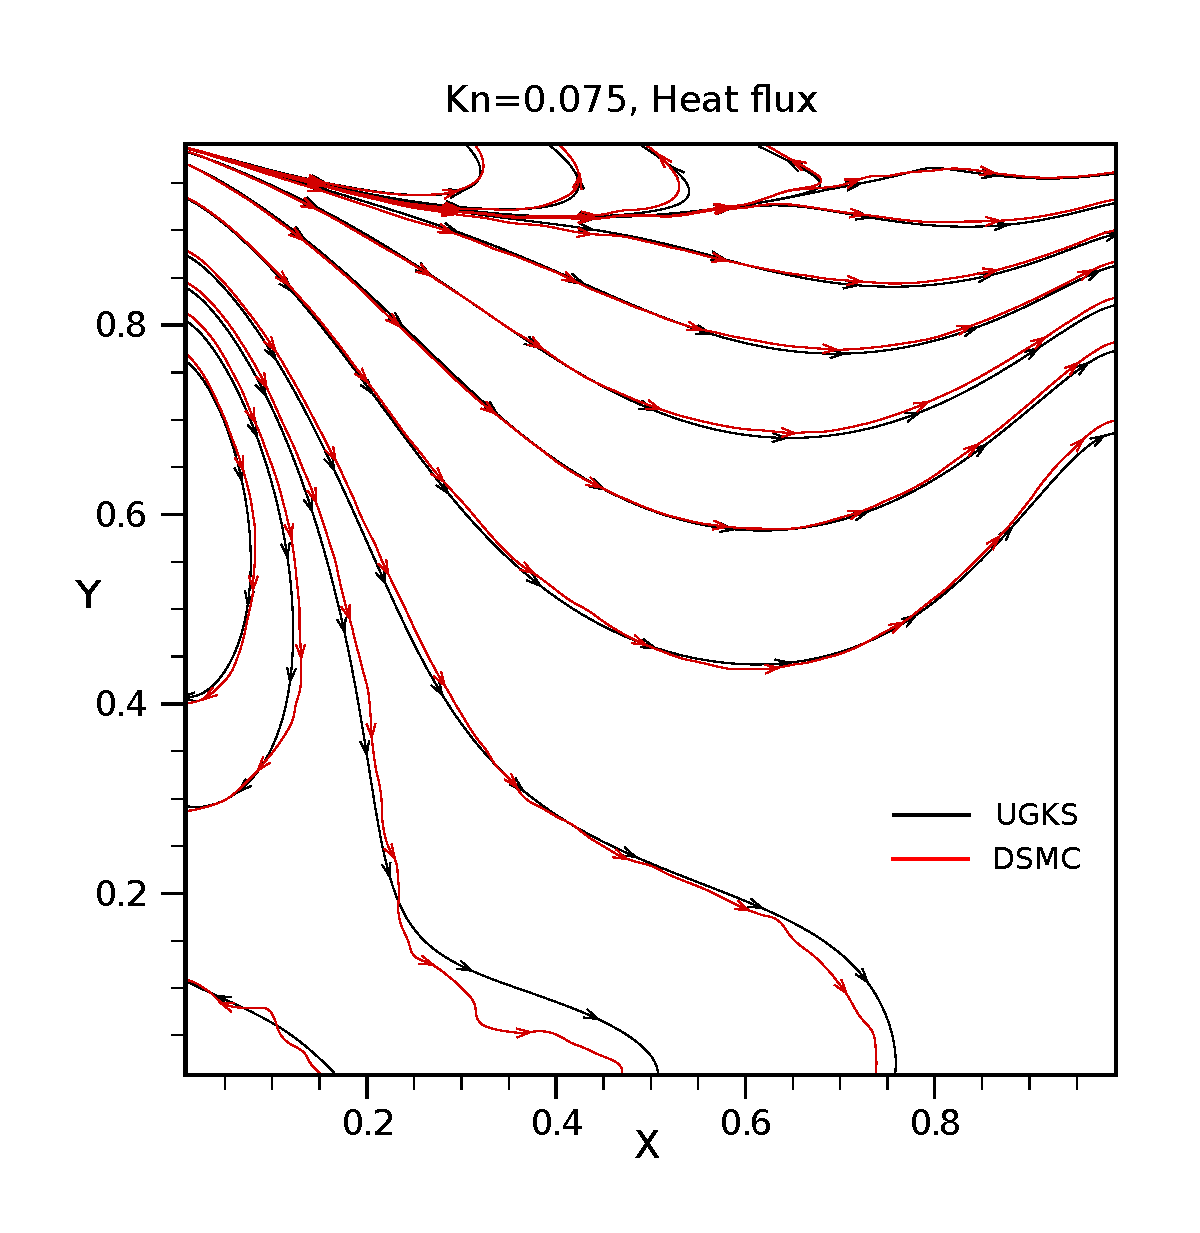
\includegraphics[width=7cm,height=6.5cm]{heatflux.eps}
    }
    \subfigure[U-velocity along vertical center line]{
        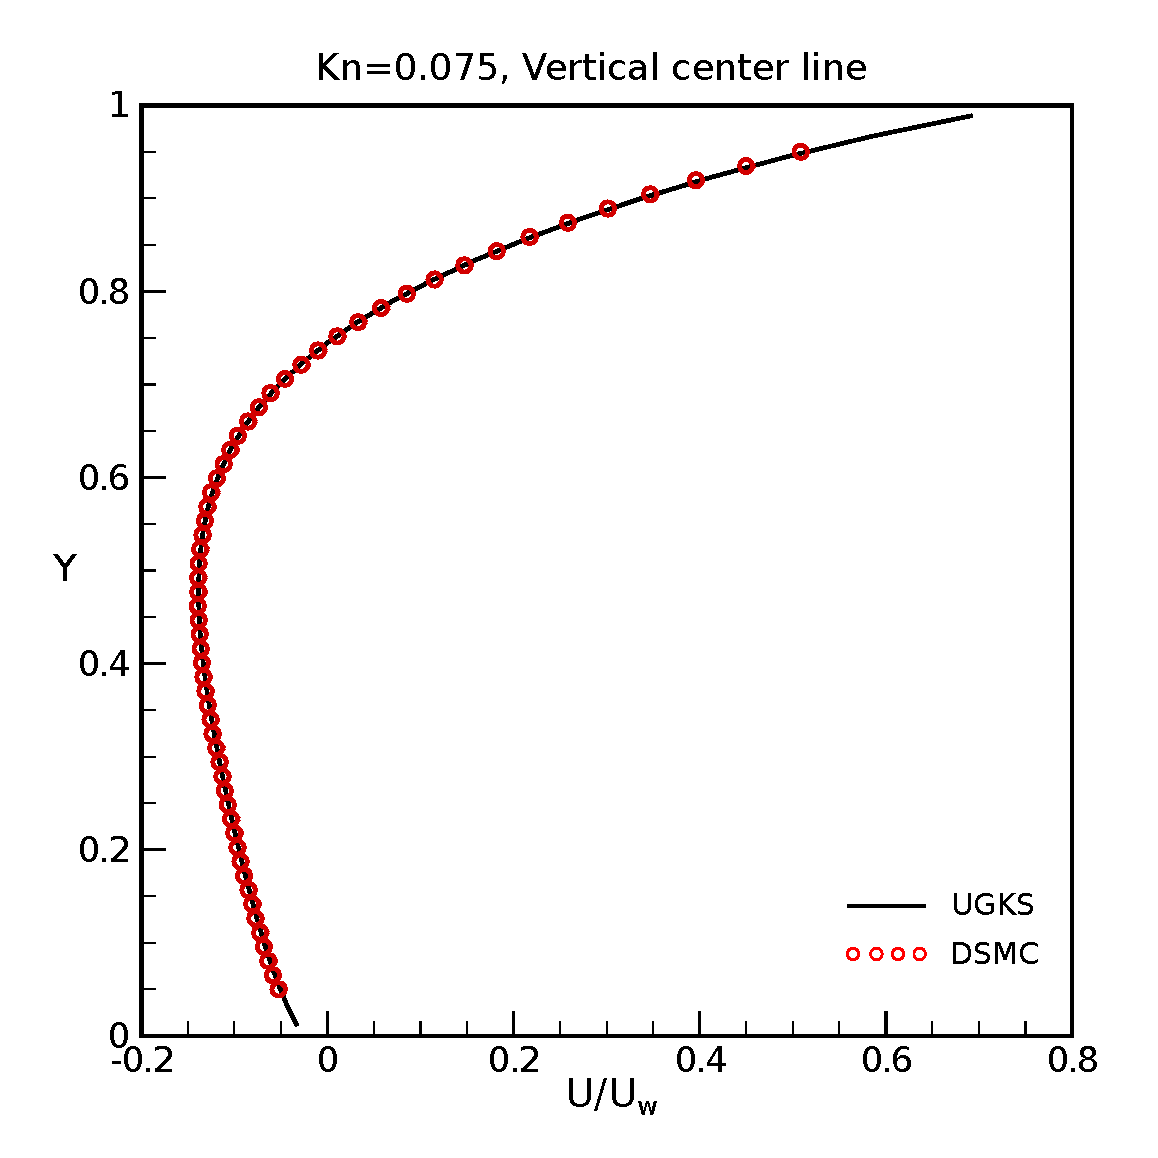
\includegraphics[width=7cm,height=6.5cm]{vline.eps}
    }
    \subfigure[V-velocity along horizontal center line]{
        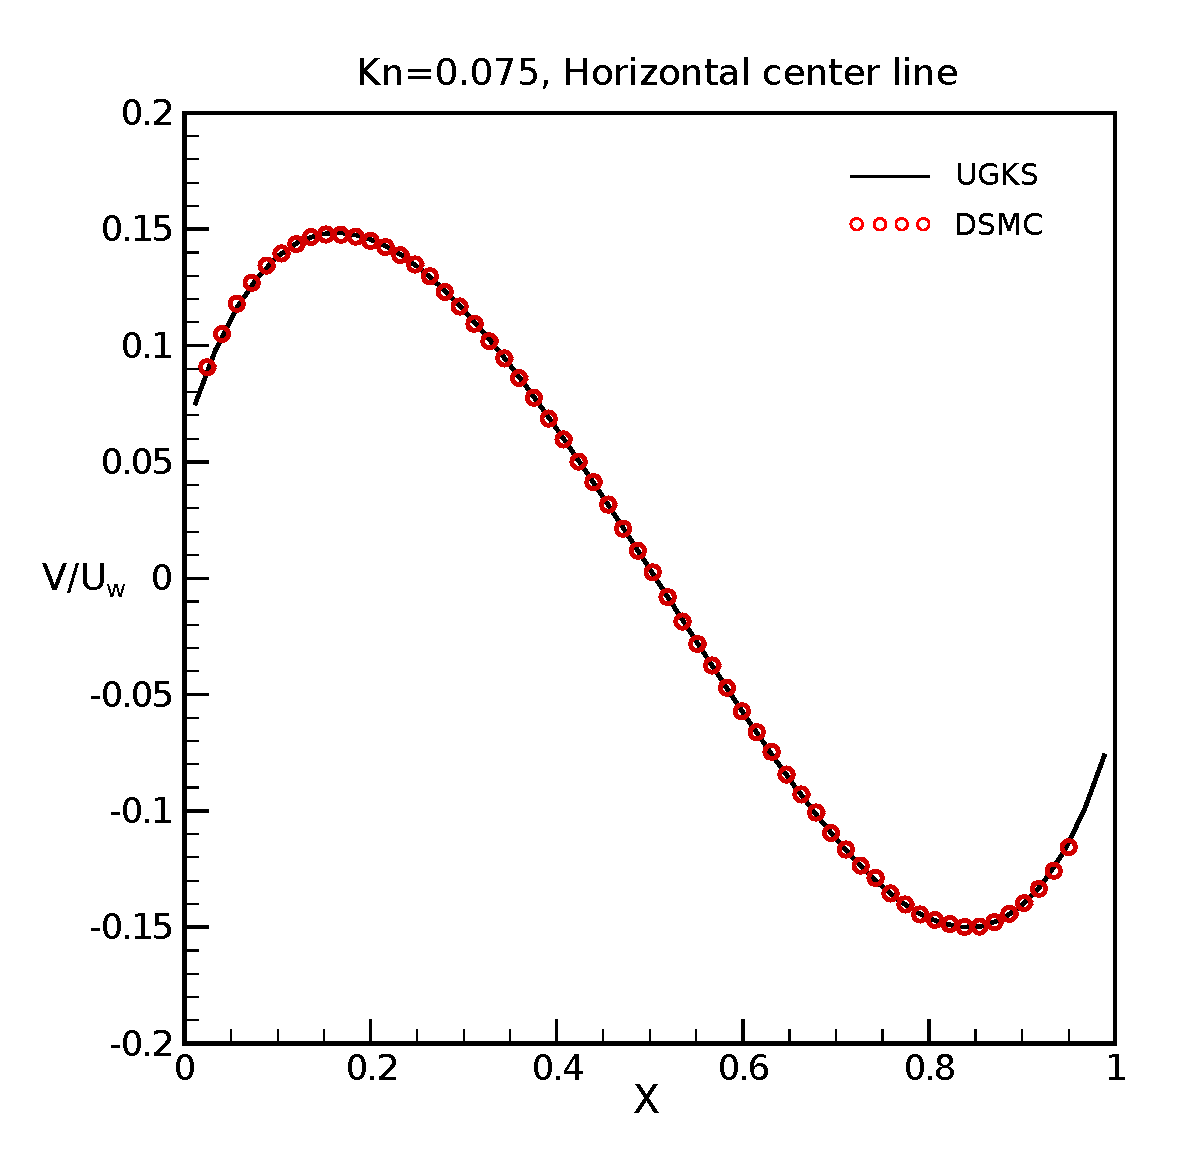
\includegraphics[width=7cm,height=6.5cm]{hline.eps}
    }
    \caption{Cavity flow at ${\rm Kn}=0.075$. In the temperature contour, the black lines are from DSMC, the white lines and background contour are from UGKS}
    \label{pic:cavity_solution}
\end{figure}

\subsection{Other information}
The Gaussian quadrature used in the code is from Table IIa of \cite{Shizgal1981}, which is better than Gaussian-Hermite quadrature in high Knudsen number. But for the cavity problem with ${\rm Kn}>=1$, Newton-Cotes formula of 61x61 velocity grids with velocity range $u,v=-4-4$ can avoid oscillating in the solution, which happens with Gaussian quadrature and second order interpolation. For example, the setting for Newton-Cotes integration

\begin{minted}{fortran}
    subroutine init()
    !variable declarations...
    real(kind=RKD) :: umin,vmin !declare smallest discrete velocity

    umin = -4.0
    vmin = -4.0
    !largest discrete velocity. Global variables
    umax = 4.0
    vmax = 4.0
    !number of velocity points. Global variables
    unum = 61
    vnum = 61

    call init_velocity_newton(unum,umin,umax,vnum,vmin,vmax) !set the velocity space
    !other commands...
    end subroutine init
\end{minted}

On Intel\textregistered\ Core\textsuperscript{\texttrademark} Quad Processor Q9450 (12M Cache, 2.66 GHz, 1333 MHz FSB) with openmp enabled, the computation time of the above setup is about 16 minutes (with openmp). With 65x65 physical space, the computation time is about 35 minutes.

%license
\backmatter
\chapter{GNU Free Documentation License}
\label{chap:fdl}

 \begin{center}

       Version 1.3, 3 November 2008


 Copyright \copyright{} 2000, 2001, 2002, 2007, 2008  Free Software Foundation, Inc.
 
 \bigskip
 
     \texttt{<http://fsf.org/>}
  
 \bigskip
 
 Everyone is permitted to copy and distribute verbatim copies
 of this license document, but changing it is not allowed.
\end{center}


\begin{center}
{\bf\large Preamble}
\end{center}

The purpose of this License is to make a manual, textbook, or other
functional and useful document ``free'' in the sense of freedom: to
assure everyone the effective freedom to copy and redistribute it,
with or without modifying it, either commercially or noncommercially.
Secondarily, this License preserves for the author and publisher a way
to get credit for their work, while not being considered responsible
for modifications made by others.

This License is a kind of ``copyleft'', which means that derivative
works of the document must themselves be free in the same sense.  It
complements the GNU General Public License, which is a copyleft
license designed for free software.

We have designed this License in order to use it for manuals for free
software, because free software needs free documentation: a free
program should come with manuals providing the same freedoms that the
software does.  But this License is not limited to software manuals;
it can be used for any textual work, regardless of subject matter or
whether it is published as a printed book.  We recommend this License
principally for works whose purpose is instruction or reference.


\begin{center}
{\Large\bf 1. APPLICABILITY AND DEFINITIONS\par}
\phantomsection
\addcontentsline{toc}{section}{1. APPLICABILITY AND DEFINITIONS}
\end{center}

This License applies to any manual or other work, in any medium, that
contains a notice placed by the copyright holder saying it can be
distributed under the terms of this License.  Such a notice grants a
world-wide, royalty-free license, unlimited in duration, to use that
work under the conditions stated herein.  The ``\textbf{Document}'', below,
refers to any such manual or work.  Any member of the public is a
licensee, and is addressed as ``\textbf{you}''.  You accept the license if you
copy, modify or distribute the work in a way requiring permission
under copyright law.

A ``\textbf{Modified Version}'' of the Document means any work containing the
Document or a portion of it, either copied verbatim, or with
modifications and/or translated into another language.

A ``\textbf{Secondary Section}'' is a named appendix or a front-matter section of
the Document that deals exclusively with the relationship of the
publishers or authors of the Document to the Document's overall subject
(or to related matters) and contains nothing that could fall directly
within that overall subject.  (Thus, if the Document is in part a
textbook of mathematics, a Secondary Section may not explain any
mathematics.)  The relationship could be a matter of historical
connection with the subject or with related matters, or of legal,
commercial, philosophical, ethical or political position regarding
them.

The ``\textbf{Invariant Sections}'' are certain Secondary Sections whose titles
are designated, as being those of Invariant Sections, in the notice
that says that the Document is released under this License.  If a
section does not fit the above definition of Secondary then it is not
allowed to be designated as Invariant.  The Document may contain zero
Invariant Sections.  If the Document does not identify any Invariant
Sections then there are none.

The ``\textbf{Cover Texts}'' are certain short passages of text that are listed,
as Front-Cover Texts or Back-Cover Texts, in the notice that says that
the Document is released under this License.  A Front-Cover Text may
be at most 5 words, and a Back-Cover Text may be at most 25 words.

A ``\textbf{Transparent}'' copy of the Document means a machine-readable copy,
represented in a format whose specification is available to the
general public, that is suitable for revising the document
straightforwardly with generic text editors or (for images composed of
pixels) generic paint programs or (for drawings) some widely available
drawing editor, and that is suitable for input to text formatters or
for automatic translation to a variety of formats suitable for input
to text formatters.  A copy made in an otherwise Transparent file
format whose markup, or absence of markup, has been arranged to thwart
or discourage subsequent modification by readers is not Transparent.
An image format is not Transparent if used for any substantial amount
of text.  A copy that is not ``Transparent'' is called ``\textbf{Opaque}''.

Examples of suitable formats for Transparent copies include plain
ASCII without markup, Texinfo input format, LaTeX input format, SGML
or XML using a publicly available DTD, and standard-conforming simple
HTML, PostScript or PDF designed for human modification.  Examples of
transparent image formats include PNG, XCF and JPG.  Opaque formats
include proprietary formats that can be read and edited only by
proprietary word processors, SGML or XML for which the DTD and/or
processing tools are not generally available, and the
machine-generated HTML, PostScript or PDF produced by some word
processors for output purposes only.

The ``\textbf{Title Page}'' means, for a printed book, the title page itself,
plus such following pages as are needed to hold, legibly, the material
this License requires to appear in the title page.  For works in
formats which do not have any title page as such, ``Title Page'' means
the text near the most prominent appearance of the work's title,
preceding the beginning of the body of the text.

The ``\textbf{publisher}'' means any person or entity that distributes
copies of the Document to the public.

A section ``\textbf{Entitled XYZ}'' means a named subunit of the Document whose
title either is precisely XYZ or contains XYZ in parentheses following
text that translates XYZ in another language.  (Here XYZ stands for a
specific section name mentioned below, such as ``\textbf{Acknowledgements}'',
``\textbf{Dedications}'', ``\textbf{Endorsements}'', or ``\textbf{History}''.)  
To ``\textbf{Preserve the Title}''
of such a section when you modify the Document means that it remains a
section ``Entitled XYZ'' according to this definition.

The Document may include Warranty Disclaimers next to the notice which
states that this License applies to the Document.  These Warranty
Disclaimers are considered to be included by reference in this
License, but only as regards disclaiming warranties: any other
implication that these Warranty Disclaimers may have is void and has
no effect on the meaning of this License.


\begin{center}
{\Large\bf 2. VERBATIM COPYING\par}
\phantomsection
\addcontentsline{toc}{section}{2. VERBATIM COPYING}
\end{center}

You may copy and distribute the Document in any medium, either
commercially or noncommercially, provided that this License, the
copyright notices, and the license notice saying this License applies
to the Document are reproduced in all copies, and that you add no other
conditions whatsoever to those of this License.  You may not use
technical measures to obstruct or control the reading or further
copying of the copies you make or distribute.  However, you may accept
compensation in exchange for copies.  If you distribute a large enough
number of copies you must also follow the conditions in section~3.

You may also lend copies, under the same conditions stated above, and
you may publicly display copies.


\begin{center}
{\Large\bf 3. COPYING IN QUANTITY\par}
\phantomsection
\addcontentsline{toc}{section}{3. COPYING IN QUANTITY}
\end{center}


If you publish printed copies (or copies in media that commonly have
printed covers) of the Document, numbering more than 100, and the
Document's license notice requires Cover Texts, you must enclose the
copies in covers that carry, clearly and legibly, all these Cover
Texts: Front-Cover Texts on the front cover, and Back-Cover Texts on
the back cover.  Both covers must also clearly and legibly identify
you as the publisher of these copies.  The front cover must present
the full title with all words of the title equally prominent and
visible.  You may add other material on the covers in addition.
Copying with changes limited to the covers, as long as they preserve
the title of the Document and satisfy these conditions, can be treated
as verbatim copying in other respects.

If the required texts for either cover are too voluminous to fit
legibly, you should put the first ones listed (as many as fit
reasonably) on the actual cover, and continue the rest onto adjacent
pages.

If you publish or distribute Opaque copies of the Document numbering
more than 100, you must either include a machine-readable Transparent
copy along with each Opaque copy, or state in or with each Opaque copy
a computer-network location from which the general network-using
public has access to download using public-standard network protocols
a complete Transparent copy of the Document, free of added material.
If you use the latter option, you must take reasonably prudent steps,
when you begin distribution of Opaque copies in quantity, to ensure
that this Transparent copy will remain thus accessible at the stated
location until at least one year after the last time you distribute an
Opaque copy (directly or through your agents or retailers) of that
edition to the public.

It is requested, but not required, that you contact the authors of the
Document well before redistributing any large number of copies, to give
them a chance to provide you with an updated version of the Document.


\begin{center}
{\Large\bf 4. MODIFICATIONS\par}
\phantomsection
\addcontentsline{toc}{section}{4. MODIFICATIONS}
\end{center}

You may copy and distribute a Modified Version of the Document under
the conditions of sections 2 and 3 above, provided that you release
the Modified Version under precisely this License, with the Modified
Version filling the role of the Document, thus licensing distribution
and modification of the Modified Version to whoever possesses a copy
of it.  In addition, you must do these things in the Modified Version:

\begin{itemize}
\item[A.] 
   Use in the Title Page (and on the covers, if any) a title distinct
   from that of the Document, and from those of previous versions
   (which should, if there were any, be listed in the History section
   of the Document).  You may use the same title as a previous version
   if the original publisher of that version gives permission.
   
\item[B.]
   List on the Title Page, as authors, one or more persons or entities
   responsible for authorship of the modifications in the Modified
   Version, together with at least five of the principal authors of the
   Document (all of its principal authors, if it has fewer than five),
   unless they release you from this requirement.
   
\item[C.]
   State on the Title page the name of the publisher of the
   Modified Version, as the publisher.
   
\item[D.]
   Preserve all the copyright notices of the Document.
   
\item[E.]
   Add an appropriate copyright notice for your modifications
   adjacent to the other copyright notices.
   
\item[F.]
   Include, immediately after the copyright notices, a license notice
   giving the public permission to use the Modified Version under the
   terms of this License, in the form shown in the Addendum below.
   
\item[G.]
   Preserve in that license notice the full lists of Invariant Sections
   and required Cover Texts given in the Document's license notice.
   
\item[H.]
   Include an unaltered copy of this License.
   
\item[I.]
   Preserve the section Entitled ``History'', Preserve its Title, and add
   to it an item stating at least the title, year, new authors, and
   publisher of the Modified Version as given on the Title Page.  If
   there is no section Entitled ``History'' in the Document, create one
   stating the title, year, authors, and publisher of the Document as
   given on its Title Page, then add an item describing the Modified
   Version as stated in the previous sentence.
   
\item[J.]
   Preserve the network location, if any, given in the Document for
   public access to a Transparent copy of the Document, and likewise
   the network locations given in the Document for previous versions
   it was based on.  These may be placed in the ``History'' section.
   You may omit a network location for a work that was published at
   least four years before the Document itself, or if the original
   publisher of the version it refers to gives permission.
   
\item[K.]
   For any section Entitled ``Acknowledgements'' or ``Dedications'',
   Preserve the Title of the section, and preserve in the section all
   the substance and tone of each of the contributor acknowledgements
   and/or dedications given therein.
   
\item[L.]
   Preserve all the Invariant Sections of the Document,
   unaltered in their text and in their titles.  Section numbers
   or the equivalent are not considered part of the section titles.
   
\item[M.]
   Delete any section Entitled ``Endorsements''.  Such a section
   may not be included in the Modified Version.
   
\item[N.]
   Do not retitle any existing section to be Entitled ``Endorsements''
   or to conflict in title with any Invariant Section.
   
\item[O.]
   Preserve any Warranty Disclaimers.
\end{itemize}

If the Modified Version includes new front-matter sections or
appendices that qualify as Secondary Sections and contain no material
copied from the Document, you may at your option designate some or all
of these sections as invariant.  To do this, add their titles to the
list of Invariant Sections in the Modified Version's license notice.
These titles must be distinct from any other section titles.

You may add a section Entitled ``Endorsements'', provided it contains
nothing but endorsements of your Modified Version by various
parties---for example, statements of peer review or that the text has
been approved by an organization as the authoritative definition of a
standard.

You may add a passage of up to five words as a Front-Cover Text, and a
passage of up to 25 words as a Back-Cover Text, to the end of the list
of Cover Texts in the Modified Version.  Only one passage of
Front-Cover Text and one of Back-Cover Text may be added by (or
through arrangements made by) any one entity.  If the Document already
includes a cover text for the same cover, previously added by you or
by arrangement made by the same entity you are acting on behalf of,
you may not add another; but you may replace the old one, on explicit
permission from the previous publisher that added the old one.

The author(s) and publisher(s) of the Document do not by this License
give permission to use their names for publicity for or to assert or
imply endorsement of any Modified Version.


\begin{center}
{\Large\bf 5. COMBINING DOCUMENTS\par}
\phantomsection
\addcontentsline{toc}{section}{5. COMBINING DOCUMENTS}
\end{center}


You may combine the Document with other documents released under this
License, under the terms defined in section~4 above for modified
versions, provided that you include in the combination all of the
Invariant Sections of all of the original documents, unmodified, and
list them all as Invariant Sections of your combined work in its
license notice, and that you preserve all their Warranty Disclaimers.

The combined work need only contain one copy of this License, and
multiple identical Invariant Sections may be replaced with a single
copy.  If there are multiple Invariant Sections with the same name but
different contents, make the title of each such section unique by
adding at the end of it, in parentheses, the name of the original
author or publisher of that section if known, or else a unique number.
Make the same adjustment to the section titles in the list of
Invariant Sections in the license notice of the combined work.

In the combination, you must combine any sections Entitled ``History''
in the various original documents, forming one section Entitled
``History''; likewise combine any sections Entitled ``Acknowledgements'',
and any sections Entitled ``Dedications''.  You must delete all sections
Entitled ``Endorsements''.

\begin{center}
{\Large\bf 6. COLLECTIONS OF DOCUMENTS\par}
\phantomsection
\addcontentsline{toc}{section}{6. COLLECTIONS OF DOCUMENTS}
\end{center}

You may make a collection consisting of the Document and other documents
released under this License, and replace the individual copies of this
License in the various documents with a single copy that is included in
the collection, provided that you follow the rules of this License for
verbatim copying of each of the documents in all other respects.

You may extract a single document from such a collection, and distribute
it individually under this License, provided you insert a copy of this
License into the extracted document, and follow this License in all
other respects regarding verbatim copying of that document.


\begin{center}
{\Large\bf 7. AGGREGATION WITH INDEPENDENT WORKS\par}
\phantomsection
\addcontentsline{toc}{section}{7. AGGREGATION WITH INDEPENDENT WORKS}
\end{center}


A compilation of the Document or its derivatives with other separate
and independent documents or works, in or on a volume of a storage or
distribution medium, is called an ``aggregate'' if the copyright
resulting from the compilation is not used to limit the legal rights
of the compilation's users beyond what the individual works permit.
When the Document is included in an aggregate, this License does not
apply to the other works in the aggregate which are not themselves
derivative works of the Document.

If the Cover Text requirement of section~3 is applicable to these
copies of the Document, then if the Document is less than one half of
the entire aggregate, the Document's Cover Texts may be placed on
covers that bracket the Document within the aggregate, or the
electronic equivalent of covers if the Document is in electronic form.
Otherwise they must appear on printed covers that bracket the whole
aggregate.


\begin{center}
{\Large\bf 8. TRANSLATION\par}
\phantomsection
\addcontentsline{toc}{section}{8. TRANSLATION}
\end{center}


Translation is considered a kind of modification, so you may
distribute translations of the Document under the terms of section~4.
Replacing Invariant Sections with translations requires special
permission from their copyright holders, but you may include
translations of some or all Invariant Sections in addition to the
original versions of these Invariant Sections.  You may include a
translation of this License, and all the license notices in the
Document, and any Warranty Disclaimers, provided that you also include
the original English version of this License and the original versions
of those notices and disclaimers.  In case of a disagreement between
the translation and the original version of this License or a notice
or disclaimer, the original version will prevail.

If a section in the Document is Entitled ``Acknowledgements'',
``Dedications'', or ``History'', the requirement (section~4) to Preserve
its Title (section~1) will typically require changing the actual
title.


\begin{center}
{\Large\bf 9. TERMINATION\par}
\phantomsection
\addcontentsline{toc}{section}{9. TERMINATION}
\end{center}


You may not copy, modify, sublicense, or distribute the Document
except as expressly provided under this License.  Any attempt
otherwise to copy, modify, sublicense, or distribute it is void, and
will automatically terminate your rights under this License.

However, if you cease all violation of this License, then your license
from a particular copyright holder is reinstated (a) provisionally,
unless and until the copyright holder explicitly and finally
terminates your license, and (b) permanently, if the copyright holder
fails to notify you of the violation by some reasonable means prior to
60 days after the cessation.

Moreover, your license from a particular copyright holder is
reinstated permanently if the copyright holder notifies you of the
violation by some reasonable means, this is the first time you have
received notice of violation of this License (for any work) from that
copyright holder, and you cure the violation prior to 30 days after
your receipt of the notice.

Termination of your rights under this section does not terminate the
licenses of parties who have received copies or rights from you under
this License.  If your rights have been terminated and not permanently
reinstated, receipt of a copy of some or all of the same material does
not give you any rights to use it.


\begin{center}
{\Large\bf 10. FUTURE REVISIONS OF THIS LICENSE\par}
\phantomsection
\addcontentsline{toc}{section}{10. FUTURE REVISIONS OF THIS LICENSE}
\end{center}


The Free Software Foundation may publish new, revised versions
of the GNU Free Documentation License from time to time.  Such new
versions will be similar in spirit to the present version, but may
differ in detail to address new problems or concerns.  See
\texttt{http://www.gnu.org/copyleft/}.

Each version of the License is given a distinguishing version number.
If the Document specifies that a particular numbered version of this
License ``or any later version'' applies to it, you have the option of
following the terms and conditions either of that specified version or
of any later version that has been published (not as a draft) by the
Free Software Foundation.  If the Document does not specify a version
number of this License, you may choose any version ever published (not
as a draft) by the Free Software Foundation.  If the Document
specifies that a proxy can decide which future versions of this
License can be used, that proxy's public statement of acceptance of a
version permanently authorizes you to choose that version for the
Document.


\begin{center}
{\Large\bf 11. RELICENSING\par}
\phantomsection
\addcontentsline{toc}{section}{11. RELICENSING}
\end{center}


``Massive Multiauthor Collaboration Site'' (or ``MMC Site'') means any
World Wide Web server that publishes copyrightable works and also
provides prominent facilities for anybody to edit those works.  A
public wiki that anybody can edit is an example of such a server.  A
``Massive Multiauthor Collaboration'' (or ``MMC'') contained in the
site means any set of copyrightable works thus published on the MMC
site.

``CC-BY-SA'' means the Creative Commons Attribution-Share Alike 3.0
license published by Creative Commons Corporation, a not-for-profit
corporation with a principal place of business in San Francisco,
California, as well as future copyleft versions of that license
published by that same organization.

``Incorporate'' means to publish or republish a Document, in whole or
in part, as part of another Document.

An MMC is ``eligible for relicensing'' if it is licensed under this
License, and if all works that were first published under this License
somewhere other than this MMC, and subsequently incorporated in whole
or in part into the MMC, (1) had no cover texts or invariant sections,
and (2) were thus incorporated prior to November 1, 2008.

The operator of an MMC Site may republish an MMC contained in the site
under CC-BY-SA on the same site at any time before August 1, 2009,
provided the MMC is eligible for relicensing.


\begin{center}
{\Large\bf ADDENDUM: How to use this License for your documents\par}
\phantomsection
\addcontentsline{toc}{section}{ADDENDUM: How to use this License for your documents}
\end{center}

To use this License in a document you have written, include a copy of
the License in the document and put the following copyright and
license notices just after the title page:

\bigskip
\begin{quote}
    Copyright \copyright{}  YEAR  YOUR NAME.
    Permission is granted to copy, distribute and/or modify this document
    under the terms of the GNU Free Documentation License, Version 1.3
    or any later version published by the Free Software Foundation;
    with no Invariant Sections, no Front-Cover Texts, and no Back-Cover Texts.
    A copy of the license is included in the section entitled ``GNU
    Free Documentation License''.
\end{quote}
\bigskip
    
If you have Invariant Sections, Front-Cover Texts and Back-Cover Texts,
replace the ``with \dots\ Texts.''\ line with this:

\bigskip
\begin{quote}
    with the Invariant Sections being LIST THEIR TITLES, with the
    Front-Cover Texts being LIST, and with the Back-Cover Texts being LIST.
\end{quote}
\bigskip
    
If you have Invariant Sections without Cover Texts, or some other
combination of the three, merge those two alternatives to suit the
situation.

If your document contains nontrivial examples of program code, we
recommend releasing these examples in parallel under your choice of
free software license, such as the GNU General Public License,
to permit their use in free software.


%appendix
\begin{appendices}
    \setcounter{chapter}{1}

    %moments of maxwell
    \appxchapter{Moments of Maxwellian distribution function}
    \label{appendix:moments}
    In the program, the moments of Maxwellian distribution function is frequently used, and they are usually obtained from subroutines.

    The moments of Maxwellian distribution function is defined as
    $$\rho<...>=\int(...)gd\Xi$$
    and have the property that
    $$<u^n \xi^m> = <u^n><\xi^m>$$
    where $m,n$ are integers.

    \section*{Moments of $\xi^m$}
    $$<\xi^2>=\left(\frac{K}{2\lambda}\right),\quad <\xi^4>=\left(\frac{3K}{4\lambda^2}+\frac{K(K-1)}{4\lambda^2}\right)$$

    \section*{Moments of $u^n$}
    The integration limits of $<u^n>$ is from $-\infty$ to $\infty$
    $$
    \begin{aligned}
        <u^0> &= 1\\
        <u^1> &= U\\
        <u^{n+2}> &= U<u^{n+1}>+\frac{n+1}{2\lambda}<u^n>
    \end{aligned} 
    $$
    The integration limits of $<u^n>_{>0}$ is from $0$ to $\infty$,
    $$
    \begin{aligned}
        <u^0>_{>0} &= \frac{1}{2}{\rm erfc}(-\sqrt{\lambda}U) \\
        <u^1>_{>0} &= U<u^0>_{>0}+\frac{1}{2}\frac{e^{-\lambda U^2}}{\sqrt{\pi\lambda}} \\
        <u^{n+2}>_{>0} &= U<u^{n+1}>_{>0}+\frac{n+1}{2\lambda}<u^n>_{>0}
    \end{aligned} 
    $$
    The integration limits of $<u^n>_{<0}$ is from $-\infty$ to $0$,
    $$
    \begin{aligned}
        <u^0>_{<0} &= \frac{1}{2}{\rm erfc}(\sqrt{\lambda}U) \\
        <u^1>_{<0} &= U<u^0>_{<0}-\frac{1}{2}\frac{e^{-\lambda U^2}}{\sqrt{\pi\lambda}} \\
        <u^{n+2}>_{<0} &= U<u^{n+1}>_{<0}+\frac{n+1}{2\lambda}<u^n>_{<0}
    \end{aligned} 
    $$

    \section*{Moments of $<u^n\xi^m\psi>$}
    There are three components for 1D problem
    $$
    <u^n\xi^m\psi>=\begin{pmatrix}
        <u^n><\xi^m>\\
        <u^{n+1}><\xi^m>\\
        \frac{1}{2}\left(<u^{n+2}><\xi^m>+<u^n><\xi^{m+2}>\right)
    \end{pmatrix} 
    $$

    \section*{Moments of $<au^n\psi>$}
    There are three components for 1D problem
    $$<au^n\psi>=a_1<u^n\psi>+a_2<u^{n+1}\psi>+\frac{1}{2}a_3\left(<u^{n+2}\psi>+<u^n\xi^2\psi>\right)$$
\end{appendices}

%References
\cleardoublepage
\phantomsection
\addcontentsline{toc}{chapter}{Bibliography}
\bibliographystyle{unsrt}
\bibliography{manual}
\end{document}
